\section{Die Tschebyscheff-Polynome}
\begin{defn}
Die \emph{Tschebyscheff-Polynome} $ T_m(z) $ sind gegeben durch die Rekursion
\[
T_{m+1}(z)=2zT_m(z)-T_{m-1}(z), \quad m \ge 1,
\]
mit
\[
T_0(z)=1, \quad T_1(z)=z.
\]
Es ist bekannt: Die $T_m(z)$ sind Orthogonalpolynome bez�glich des Innenproduktes
\[
\langle  p,q\rangle  = \int_{-1}^{1} \frac{1}{\sqrt{1-x^2}}p(x)q(x)\ dx, \quad \text{ auf $\Pi$= Menge der Polynome.}
\]
\end{defn}

\begin{sa}
Die L�sung $p_m$ der Minimierungsaufgabe
\[
\underset{p_m \in \Pi_m, p_m(c)=1}{\min}\quad \underset{\lambda \in [-1,1]}{\max} |p_m(\lambda)|,
\]
f�r $c \notin [-1,1]$ lautet
\[
p_m(z) = \frac{1}{T_m(c)} T_m(z).
\]
\end{sa}
\begin{proof}
Siehe Vorlesung: Parallele Algorithmen (Vorlesung im Wintersemester 2002/03, Abschnitt 4.4).
\end{proof}

\medskip

Wir interessieren uns nun f�r Optimalpolynome auf etwas allgemeineren Gebieten, n"amlich Ellipsen.

\begin{defn}
F"ur $\rho \geq 1$ sei $E_{\rho}$ die Ellipse mit Brennpunkten in $-1$ und $+1$ und 
mit gro\ss{}er Halbachse $a=(1/2)\cdot(\rho + 1/\rho)$ und kleiner Halbachse $b=(1/2)\cdot
(\rho-1/\rho)$.
Die "`Schnurl�nge"' $\mu$ betr"agt also $\rho + 1/\rho$. 
\begin{center}

\begin{tikzpicture}

 \draw[->]        (0,-3)   -- (0,3);
 \draw[->]        (-6,0)   -- (6,0);
 
\draw (0, 0) ellipse (4 and 2);
\coordinate[label=below:$F1$] (A) at (-3.46,0);
\coordinate[label=below:$F2$] (B) at (3.46,0);
\coordinate[label=right:$P$] (C) at (3,1.32);
\draw (A) -- (C) -- (B);
\coordinate (D) at ($(A)!0.5!(C)$);
\coordinate (E) at ($(B)!0.5!(C)$);
\coordinate[label=above:$\mu$] (F) at (2,2.5);
\draw (D) -- (F) -- (E) ;

\fill[gray] (A) circle (2pt);
\fill[gray] (B) circle (2pt);
\fill[gray] (C) circle (2pt);


%\coordinate[label=90:$D$] (D) at ($(C)!1cm!90:(B)$);
%\draw (C) -- (D) node[midway, sloped, above] {1cm};
%\coordinate (midone) at ($(A)!0.5!(C)$);
%\node at (midone){\textcolor {red}{$\times$}}


\draw [
    thick,
    decoration={
        brace,
        mirror,
        raise=0.5cm
    },
    decorate
] (0,0) -- (4,0) 
node [pos=0.5,anchor=north,yshift=-0.55cm] {a};


\draw [
    thick,
    decoration={
        brace,
%        mirror,
        raise=0.5cm
    },
    decorate
] (0,0) -- (0,2) 
node [pos=0.5,anchor=west,xshift=-1.2cm] {b};
\end{tikzpicture}


%\begin{picture}(240,140)
%\put(110,60){\ellipse{200}{104}}						% Kommando aus eepic
%\put(160,60){\circle*{4}}
%\put(60,60){\circle*{4}}
%\put(0,60){\vector(1,0){240}}
%\put(110,0){\vector(0,1){140}}
%\drawline(60,60)(130,111)(160,60)						% Kommando aus eepic
%\put(112,60){$\underbrace{\hspace*{98pt}}_{\textstyle a}$}			% Bi�chen gemogelt
%\put(95,30){$b \left\{ \begin{array}{c}\vspace*{34pt}\end{array} \right.$}	% noch mehr gemogelt

%\thicklines									% Dicke Linie an
%\drawline(90,80)(200,120)(150,80)
%\put(202,120){$\mu$}
%\end{picture}
\end{center}
\end{defn}

Die hier gegebene Definition einer Ellipse "uber ihre Brennpunkte und den Parameter $\rho$
ist nicht Standard. Man rechnet aber einfach nach, dass so tats"achlich eine Ellipse 
gegeben ist, indem man nachweist, dass die Summe der Abst"ande zu den beiden Brennpunkten
f"ur jeden Punkt auf $E_\rho$ gerade die Schnurl"ange $\mu$ ist. 

\begin{defn}
Die \emph{Joukowski-Abbildung} $J:\co \setminus \{0\} \lr \co$ ist definiert durch
\[
J(w) = \frac{1}{2}(w+w^{-1}).
\]
\end{defn}

Mit Hilfe dieser Abbildung wollen wir Folgendes zeigen:

\begin{lem} Es ist
$J(D(0,\rho)) = E_{\rho}$. 
\end{lem}
\begin{proof}
Wir stellen als erstes die Gleichung f�r $E_{\rho}$ auf $(z = x + iy)$:
\[
\frac{x^2}{\left(\frac{\rho+1/\rho}{2}\right)^2} + \frac{y^2}{\left(\frac{\rho-1/\rho}{2}\right)^2} = 1.
\]
Eine Parametrisierung von $E_{\rho}$ ist dann
\[
x(t) = \frac{\rho+1/\rho}{2} \cdot \cos t, \enspace 
y(t) = \frac{\rho-1/\rho}{2} \cdot \sin t
\]
mit $t \in [0, 2\pi)$. Dann gilt
\begin{align*}
x^2(t)+y^2(t)&=\left(\frac{\rho+1/\rho}{2}\right)^2 \cos^2 t + \left(\frac{\rho-1/\rho}{2}\right)^2 \sin^2 t \\
&=\frac{1}{4}\left(\rho+(1/\rho)\right)^2 - \sin^2 t.
\end{align*}
Andererseits gilt mit $w=\rho e^{i\theta} \in D(0,\rho)$ f"ur das Bild
$z=J(w)=\frac{1}{2}(w+w^{-1})$
\begin{align*}
z \overline{z} &= \frac{1}{4} (w+w^{-1})(\overline{w}+\overline{w}^{-1}) \\
&= \frac{1}{4}(w \overline{w} + w^{-1} \overline{w} + w \overline{w}^{-1} + w^{-1}\overline{w}^{-1}) \\
&= \frac{1}{4}\left(\rho^2 + e^{-2i \theta} + e^{2i\theta} + \frac{1}{\rho^2}\right) \\
&= \frac{1}{4}\left(\rho^2 + 2 \cos(2\theta) + \frac{1}{\rho^2}\right) \\
&= \frac{1}{4}\left(\rho^2 - 4 \sin^2(\theta) + 2 + \frac{1}{\rho^2}\right) \\
&= \frac{1}{4}\left(\rho^2 + 2 + \frac{1}{\rho^2}\right) - \sin^2(\theta) \\
&= \frac{1}{4}\left(\rho + \frac{1}{\rho}\right)^2 - \sin^2(\theta). 
\end{align*}
Vergleich mit der Parameterdarstellung ergibt einfach 
\[
\theta = t.
\]
\end{proof}

Die Gleichung $z = J(w) = \frac{1}{2}(w + w^{-1})$ hat zwei L�sungen $w$, 
die zueinander invers sind.
Sei nun $w(z)$ eine dieser L�sungen z.B. die betragsm��ig gr��ere.

\begin{lem} \label{tscheby_lem}
Es gilt
\[
T_m(z)=\left[ \frac{1}{2}\left( w^m(z) + w^{-m}(z) \right) \right].
\]
\end{lem}
\begin{proof}
Wir beweisen dies nat�rlich �ber die Rekursionsformel. F�r $m=0,1$ ist die Behauptung 
offensichtlich richtig und per Induktion gilt
\begin{align*}
T_{m+1}(z) &= z\left( w^m(z) + w^{-m}(z) \right) - \frac{1}{2}\left( w^{m-1}(z) + w^{-(m-1)}(z) \right) \\
&= \frac{1}{2} \left( w(z) + w^{-1}(z) \right)\left( w^m(z) + w^{-m}(z) \right)\\
& \phantom{= z\left( w^m(z) + w^{-m}(z) \right)}
				-\frac{1}{2}\left( w^{m-1}(z) + w^{-(m-1)}(z) \right) \\
&= \frac{1}{2}\left( w^{m+1}(z) + w^{-(m+1)}(z) \right).
\end{align*}
\end{proof}

Betrachtet wird nun die MinMax-Aufgabe
\begin{equation} \label{minmaxell_eq}
\underset{p \in \Pi_m, p(\gamma) = 1}{\min} \quad  \underset{\lambda \in E_{\rho}}
\max |p(\lambda)| \quad \text{f�r } \gamma \notin E_{\rho}.
\end{equation}

\begin{sa}\label{cmschranke_sa}
Sei $c_m$ der Wert des Minimums in \eqnref{minmaxell_eq} 
und $\gamma = \frac{1}{2}(w_{\gamma} + w_{\gamma}^{-1})$, 
wobei $w_{\gamma}$ die betragsm��ig gr��ere der beiden m�glichen L�sungen ist.
Dann gilt
\[
\frac{\rho^m}{|w_{\gamma}|^m} \le c_m \le \frac{1}{|w_{\gamma}^m+w_{\gamma}^{-m}|}\left(\rho^m + \left(\frac{1}{\rho}\right)^m \right),
\]
wobei die obere Schranke f"ur das Polynom 
\[
p^*_m(z) = \frac{1}{T_m(\gamma)} T_m(z)
\]
erreicht wird.
\end{sa}
\begin{proof}
Wir stellen ein beliebiges Polynom $p_m \in \overline{\Pi}_m$ in der Basis der Tschebyscheff-Polynome dar, d.h.
\[
p_m = \sum\limits_{\nu=0}^{m} a_{\nu}T_{\nu}.
\]
Wegen $p_m(\gamma) = 1$ gilt $1 = \sum\limits_{\nu=0}^{m} a_{\nu}T_{\nu}(\gamma)$. Unter
Verwendung von $w = w(z)$ wie im Lemma \nref{tscheby_lem} ergibt sich
\begin{align*}
p_m(z) &= \sum\limits_{\nu=0}^{m} a_{\nu}\left( \frac{1}{2}\left( w^{\nu} + w^{-\nu} \right) \right) \\
&= \sum\limits_{\nu=0}^{m} a^{'}_{\nu}\left( \frac{\frac{1}{2}\left( w^{\nu} + w^{-\nu} \right)}{\frac{1}{2}\left( w_{\gamma}^{\nu} 
		+ w_{\gamma}^{-\nu} \right)} \right).
\end{align*}

Hierin ist $\sum\limits_{\nu=0}^{m} a^{'}_{\nu} = 1$. W"ahlen wir speziell
$a^{'}_m = 1$, $a^{'}_{\nu} = 0$ ,$ \nu = 0,...,m-1$,
also
\[
 p_m(z) = p_m^*(z) = \frac{1}{T_m(\gamma)} T_m(z) = \frac{w^m + w^{-m} }{ w_{\gamma}^m + w_{\gamma}^{-m} }, 
\]
so gilt wegen des Maximums-Prinzips 
\begin{align*}
\underset{z \in E_{\mu} }{\max} |p_m^*(z)|&=\underset{z \in \partial E_{\mu} }{\max} |p_m^*(z)| \\
&= \underset{w \in \partial D(0,\rho)}{\max} \left| \frac{w^m + w^{-m} }{ w_{\gamma}^m + w_{\gamma}^{-m} } \right| \\
&= \frac{1}{|w_{\gamma}^m + w_{\gamma}^{-m}|} \left[ \rho^m + \left(\frac{1}{\rho}\right)^m\right].
\end{align*}
Die letzte Gleichheit ist richtig, weil $|w^m + w^{-m}| \leq |w^m| + |w^{-m}| =
|\rho^m| + |\rho^{-m}|$,
und diese obere Schranke wird f"ur $w = \rho$ auch angenommen.

F�r die Bestimmung einer unteren Schranke sei das Optimalpolynom $\widetilde{p}_m(z)$
dargestellt durch 
\begin{align*}
\widetilde{p}_m(z) 
&= \sum\limits_{\nu=0}^{m} b_{\nu}\left(\frac{w^{\nu}+w^{-\nu}}{w_{\gamma}^{\nu} 
		+ w_{\gamma}^{-\nu}} \right), \quad \quad \sum\limits_{\nu=0}^{m} b_{\nu}=1 \\
&= \left( \frac{ w^{-m} }{ w_{\gamma}^{-m} } \right) \underbrace{ \sum\limits_{\nu=0}^{m} b_{\nu}
		 \left( \frac{ w^{\nu+m} + w^{-\nu+m} }{ w_{\gamma}^{\nu+m} + w_{\gamma}^{-\nu+m} } \right)}_{\text{Polynom $q$ 
				vom Grad $2m$ in $w$, $q(w_\gamma)=1$}}.
\end{align*}
Nach Satz \nref{Minmaxkreis_sa} gilt 
\[
\underset{w \in D(0,\rho)}{\max} \left| \sum\limits_{\nu=0}^{m} b_{\nu} \left( \frac{ w^{\nu+m} + w^{-\nu+m} }{ w_{\gamma}^{\nu+m} 
		+ w_{\gamma}^{-\nu+m} } \right)\right| \ge \left( \frac{\rho}{|w_{\gamma}|}\right)^{2m},
\]
falls $w_{\gamma}$ die betragsm��ig gr��ere L�sung ist (und damit au"serhalb von $D(0,\rho)$ liegt).
Also gilt
\[
\left| \widetilde{p}_m(z) \right| \ge \left| \frac{w^{-m}}{w_{\gamma}^{-m}}\right| \left(\frac{\rho}{|w_{\gamma}|}\right)^{2m} 
= \frac{\left| w^{-m} \right| \rho^{2m}}{\left| w_{\gamma} \right|^{m}}
= \frac{\rho^m}{|w_{\gamma}|^m}.
\]
\end{proof}

\begin{bem}
F�r $\gamma \notin E_{\rho}$ gilt $|w_{\gamma}| < \rho^{-1}$ mit $\rho \ge 1$.
Also ist sowohl $\limm ( 1/\rho )^m = 0$ als auch $\limm w_{\gamma}^{-m} = 0$.
Satz \nref{cmschranke_sa} zeigt so, dass die Tschebyscheff-Polynome \emph{asymptotisch optimal} sind, aber nicht notwendig 
optimal f�r endliches $m$.
\end{bem}

\begin{aufg}
Bestimme jeweils die (im Sinne von Satz \nref{cmschranke_sa}) asymptotisch optimale L�sung der MinMax-Aufgabe
\[
\underset{p_m \in \overline{\Pi}_m }{\min} \quad \underset{\lambda \in E}{\max} |p(\lambda)|
\]
und den zugeh�rigen Wert des Minimums f�r die F�lle:
\begin{enumerate}
\item $E = a + bE_{\rho}$, wobei $a,b > 0$ und $ a - b\cdot \frac{1}{2}(\rho+1/\rho)  > 0 $\\
\begin{center}
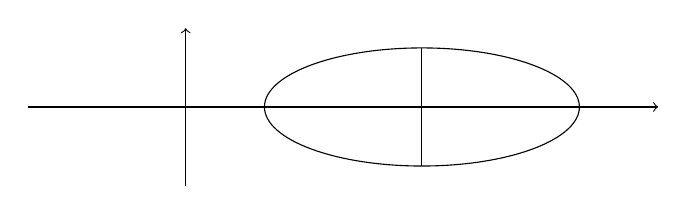
\begin{tikzpicture}
\draw[->] (-2,0) -- (6,0);
\draw[->] (0,-1) -- (0,1);
\draw (3,0) ellipse (2 and 0.75);
\draw (3,-0.75) -- (3,0.75);
\end{tikzpicture}\\
\end{center}

\item $E = a + b e^{i\frac{\pi}{2}}E_\rho$, wobei $a,b > 0$ und $a-b\cdot\frac{1}{2}(\rho + \frac{1}{\rho}) > 0$\\
\begin{center}
\begin{tikzpicture}
\draw[->] (-2,0) -- (6,0);
\draw[->] (0,-2) -- (0,2);
\draw (3,0) ellipse (0.75 and 2);
\draw (3,-2) -- (3,2);
\end{tikzpicture}\\
\end{center}

\item $E_\rho$ ist ein Geradenst�ck parallel zur reellen Achse von $-a$ bis $+a$ mit Achsenabschnitt $b$ auf der imagin�ren Achse.\\
\begin{center}
\begin{tikzpicture}
\draw[->] (-3,0) -- (3,0);
\draw[->] (0,-1) -- (0,2);
\draw (-2,1) -- (2,1);
\draw (-2,1) node[anchor=north]{$-a$};
\draw (2,1) node[anchor=north]{$+a$};
\draw (0,1) node[anchor=north west]{$b$};
\end{tikzpicture}\\
\end{center}
Sind in diesem Fall die Polynome auch optimal f"ur endliches $m$? 
\end{enumerate}
\end{aufg}

\begin{bem}
Die Optimalpolynome im Sinne von Satz \nref{cmschranke_sa} sind unabh�ngig vom Parameter
$\rho$ der Ellipse $E_\rho$ (solange $\gamma$ immer noch au�erhalb der Ellipse liegt).

\begin{figure}[h!]
\begin{center}
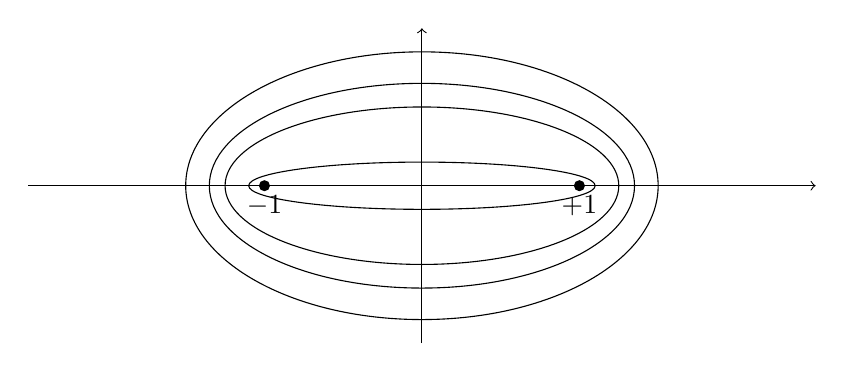
\begin{tikzpicture}
\draw[->] (-5,0) -- (5,0);
\draw[->] (0,-2) -- (0,2);

\fill (-2, 0) circle (2pt);
\fill (2, 0) circle (2pt);
\draw (-2,0) node[anchor=north]{$-1$};
\draw (2,0) node[anchor=north]{$+1$};


\draw (0,0) ellipse (2.2 and 0.3);
\draw (0,0) ellipse (2.5 and 1);
\draw (0,0) ellipse (2.7 and 1.3);
\draw (0,0) ellipse (3 and 1.7);

\end{tikzpicture}\\
\end{center}
\caption{Ellipsen $E_\rho$ f"ur verschiedene Werte von $\rho$}
\end{figure}

\noindent Aus Satz \ref{Minmaxkreis_sa} ist bekannt, dass f�r den Kreis $D(0,\rho)$ die
MinMax-Aufgabe
\[
\underset{p \in \Pi_m, p(\gamma)=1}{\min} \quad \underset{\lambda \in D(0, \rho)}{\max} \left| p_m(\lambda) \right|
\]
durch das Polynom $p_m(z)=\frac{z^m}{\gamma^m}$ gel"ost wird.
F"ur dessen Ableitungen $p_m^{(k)}(z) = m(m-1) \cdot ... \cdot (m-k+1) \frac{z^{m-k}}{\gamma^m}$ gilt
\begin{align*}
\underset{z \in D(0,\rho)}{\max} \left| p_m^{(k)}(z) \right| &= m \cdot ... \cdot (m-k+1) \frac{\rho^{m-k}}{\gamma^m} \\
&= m \cdot ... \cdot (m-k+1) \rho^{-k} \left( \frac{\rho}{\gamma} \right)^m \underset{m \to \infty}{\lr} 0,
\end{align*}
wobei die Konvergenz sogar gleichm"a�ig ist auf $D(0,\rho)$. Dies ist wichtig mit
Blick auf Satz~\ref{KonvergenzKUV_sa}
\end{bem}

F�r die Tschebyscheffpolynome und Ellipsen gilt ein entsprechendes Resultat.

\begin{sa} \label{}
Es sei $E_\rho = J(D(0,\rho))$ mit $\rho >1$ eine Ellipse.
Weiter sei $p^*_m$ das $m$-te skalierte Tschebyscheffpolynom,
$p^*_m(z)=\frac{w^m + w^{-m}}{w_{\gamma}^m+w_{\gamma}^{-m}}$, wobei
$z = J(w) = \frac{1}{2}(w + w^{-1})$ und $J(w_\gamma) = \gamma$, mit $\gamma$ au�erhalb von
$E_{\rho}$, d.h. $\left| w_{\gamma} \right| > \rho$.
Dann gilt f�r alle $k \in \mathbb{N}$
\[
\left| {p_m^*}^{(k)}(z) \right| \underset{m \to \infty}{\lr} 0 \enspace
\text{ gleichm"a�ig auf } E_\rho.
\]
\end{sa}
\begin{proof}
Beachte (im Vorgriff auf die Formulierung des Tschebyscheff-Ver\-fahr\-ens in
Algorithmus \ref{Tschebyscheff_alg}): Im Zusammenhang mit Satz~\ref{KonvergenzKUV_sa}
besagt dieser Satz, dass Diagonalisierbarkeit
f�r ein erfolgreiches Tschebyscheffverfahren nicht vorausgesetzt werden muss.

Mit
\begin{align*}
&p_m^*(z) = \frac{w^m + w^{-m}}{w_{\gamma}^m+w_{\gamma}^{-m}}, \\
&\frac{dz}{dw} = \frac{1}{2}(1-w^{-2}) \text{ und } \frac{dw}{dz} |_{z=J(w)} = \frac{2}{1-w^{-2}},
\end{align*}
erhalten wir
\begin{align*}
 \frac{dp^*_m(z)}{dw} \cdot \frac{dw}{dz} &= \frac{mw^{m-1} - mw^{-(m+1)}}{w_{\gamma}^m + w_{\gamma}^{-m}} \cdot \frac{2}{1-w^{-2}} \\
&=2 \frac{mw^{m+1} - mw^{-m+1}}{(w_{\gamma}^m + w_{\gamma}^{-m})(w^2-1)}.
\end{align*}
Der Term $s_m(w)=m \frac{w^{m+1}}{(w^2-1)(w_{\gamma}^m + w_{\gamma}^{-m})}$ wird f�r $ |w| = \rho$ abgesch�tzt durch
\[
|s_m(w)| \le m \frac{1}{\rho^2-1}\cdot\frac{\rho^{m+1}}{\left| w_{\gamma}^m + w_{\gamma}^{-m} \right|}
\le \frac{m}{\rho^2-1}\cdot\frac{\rho}{\left|
w_{\gamma}/\rho\right|^m - \left| w_{\gamma} \rho \right|^{-m}}.
\]
Hierin ist die rechte obere Schranke unabh"angig von $w \in \partial D(0,\rho)$.
Wegen des Maximumsprinzips gilt die Schranke sogar f"ur alle $w \in D(0,\rho)$,
also f"ur alle $z \in E_\rho$.  Aus
\[
 |w_\gamma / \rho| >1, \enspace |w_\gamma \rho| > 1,
\]
erkennen wir mit der Regel von de l'H\^{o}pital, dass die obere Schranke f"ur
$m \to \infty$ gegen 0 geht.
Dies beweist den Satz f"ur die erste Ableitung; f"ur h"ohere Ableitungen geht der Beweis
(induktiv) analog.
\end{proof}

